\subsection{Backdoors}


The system is running the website on a “WildFly” service, at port 8080. On the website (fakestagram), it is possible to upload images to the sever (and almost every other type of file), which will be saved, and can then be found at “http://[IP]:8080/img/”. There is also running a version of apache on the system. It is looking at the same location on the system that the files get uploaded to. \\
Therefore it is possible to upload PHP files from fakestagram, on the WildFly service, and execute the PHP with apache. \\ \\
By uploading the following PHP code:\\
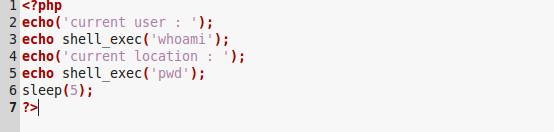
\includegraphics[width=\textwidth,height=\textheight,keepaspectratio]{code.png} \\ \\
We can see from from what user that executes the code, and from where it is being done. \\
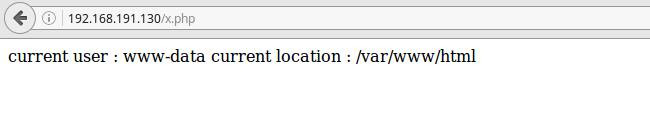
\includegraphics[width=\textwidth,height=\textheight,keepaspectratio]{exploit.png} \\ \\
If defining a backdoor as a way to gain root access to the system. Then we didn't manage to exploit any. \\
But we do believe that by poking a bit more around in the system from the remote code execution with PHP, we might have gained root access.